\uuid{ZZrO}
\exo7id{5523}
\titre{exo7 5523}
\auteur{rouget}
\organisation{exo7}
\datecreate{2010-07-15}
\isIndication{false}
\isCorrection{true}
\chapitre{Courbes planes}
\sousChapitre{Courbes paramétrées}

\contenu{
\texte{
\label{exo:routhe1}
}
\begin{enumerate}
    \item \question{(**) \textbf{L'astroïde.}
\begin{enumerate}}
\reponse{\textbf{L'astroïde.}
  \begin{enumerate}}
    \item \question{$a$ est un réel strictement positif donné. Etudier et construire la courbe de paramétrisation~:
$\left\{
\begin{array}{l}
x=a\cos^3t\\
y=a\sin^3t
\end{array}
\right.$.}
\reponse{\textbf{Domaine d'étude.}

\textbullet~Pour tout réel $t$, $M(t)$ existe.

\textbullet~Pour tout réel $t$, $M(t+2\pi)=M(t)$. Par suite, la courbe complète est obtenue quand $t$ décrit un segment de
longueur

$2\pi$ comme par exemple $[-\pi,\pi]$.

\textbullet~Pour tout réel $t$,

$$M(-t)=\left(\begin{array}{c}
\cos^3(-t)\\
\sin^3(-t)
\end{array}\right)=\left(\begin{array}{c}
\cos^3t\\
-\sin^3t
\end{array}\right)
=s_{(Ox)}(M(t)).$$

On étudie et on construit la courbe pour $t\in[0,\pi]$, puis on obtient la courbe complète par réflexion d'axe $(Ox)$.

\textbullet~Pour tout réel $t$,

$$M(t+\pi)=\left(\begin{array}{c}
\cos^3(t+\pi)\\
\sin^3(t+\pi)
\end{array}\right)=\left(\begin{array}{c}
-\cos^3t\\
-\sin^3t
\end{array}\right)
=s_O(M(t)).$$

La portion de courbe obtenue quand $t$ décrit $[-\pi,0]$ est donc aussi la symétrique par rapport à $O$ de la portion de

courbe obtenue quand $t$ décrit $[0,\pi]$. Néanmoins, cette constatation ne permet pas de réduire davantage le domaine

d'éude.

\textbullet~Pour tout réel $t$,

$$M(\pi-t)=\left(\begin{array}{c}
\cos^3(\pi-t)\\
\sin^3(\pi-t)
\end{array}\right)=\left(\begin{array}{c}
-\cos^3t\\
\sin^3t
\end{array}\right)
=s_{(Oy)}(M(t)).$$

On étudie et on construit la courbe pour $t\in\left[0,\frac{\pi}{2}\right]$, puis on obtient la courbe complète par réflexion
d'axe $(Oy)$, puis

par réflexion d'axe $(Ox)$.

\textbullet~Pour tout réel $t$,

$$M\left(\frac{\pi}{2}-t\right)=\left(\begin{array}{c}
\cos^3\left(\frac{\pi}{2}-t\right)\\
\rule{0mm}{6mm}\sin^3\left(\frac{\pi}{2}-t\right)
\end{array}\right)=\left(\begin{array}{c}
\sin^3t\\
\cos^3t
\end{array}\right)
=s_{y=x}(M(t)).$$

On étudie et on construit la courbe pour $t\in\left[0,\frac{\pi}{4}\right]$, puis on obtient la courbe complète par réflexion
d'axe la droite

d'équation $y=x$, puis d'axe $(Oy)$ et enfin d'axe $(Ox)$.\rule{0mm}{5mm}

\textbf{Variations conjointes de} $\bf{x}$ \textbf{et} $\bf{y.}$ La fonction $t\mapsto x(t)$ est strictement
décroissante sur $\left[0,\frac{\pi}{4}\right]$ et la fonction $t\mapsto y(t)$ est strictement croissante sur
$\left[0,\frac{\pi}{4}\right]$.
\textbf{Etude des points singuliers.} Pour $t\in\Rr$,

$$\overrightarrow{\frac{dM}{dt}}(t)=\left(\begin{array}{c}
-3a\cos^2t\sin t\\
3a\sin^2t\cos t
\end{array}\right)=3a\cos t\sin t\left(\begin{array}{c}
-\cos t\\
\sin t
\end{array}\right).$$
Pour tout réel $t$, le vecteur $\left(\begin{array}{c}
-\cos t\\
\sin t
\end{array}\right)$ est unitaire et n'est donc pas nul. Par suite,

$$\overrightarrow{\frac{dM}{dt}}(t)=\overrightarrow{0}\Leftrightarrow 3a\cos t\sin t=0\Leftrightarrow\cos t=0\;\mbox{ou}\;\sin t=0\Leftrightarrow
t\in\frac{\pi}{2}\Zz.$$
Les points singuliers sont donc les $M\left(\frac{k\pi}{2}\right)$, $k\in\Zz$. Pour $t\notin\frac{\pi}{2}\Zz$, $M(t)$ est un
point régulier et la tangente en $M(t)$ est dirigée par le vecteur $\left(\begin{array}{c}
-\cos t\\
\sin t
\end{array}\right)$.
Etudions alors le point singulier $M(0)$. Pour $t\in\left[-\frac{\pi}{2},\frac{\pi}{2}\right]\setminus\{0\}$,

\begin{align*}\ensuremath
\frac{y(t)-y(0)}{x(t)-x(0)}&=\frac{a\sin^3t}{a\cos^3t-a}=\frac{\sin^3t}{(\cos t-1)(\cos^2t+\cos t+1)}\\
 &=\frac{8\sin^3\frac{t}{2}\cos^3\frac{t}{2}}{-2\sin^2\frac{t}{2}(\cos^2t+\cos t+1)}
=\frac{-4\sin\frac{t}{2}\cos^3\frac{t}{2}}{\cos^2t+\cos t+1},
\end{align*}
et donc, $\lim_{t\rightarrow 0}\frac{y(t)-y(0)}{x(t)-x(0)}=0$.
(Si on connaît déjà les équivalents, c'est plus court :  $\frac{\sin^3t}{(\cos t-1)(\cos^2t+\cos t+1)}\underset{x\rightarrow0}{\sim}\frac{t^3}{-\frac{t^2}{2}\times3}=-\frac{2t}{3}\rightarrow0$). La courbe admet en $M(0)$ une tangente dirigée par le vecteur
$(1,0)$. Par symétrie, la courbe admet également une tangente en $M\left(-\frac{\pi}{2}\right)$, $M\left(\frac{\pi}{2}\right)$ et $M(\pi)$,
dirigée respectivement par $(0,1)$, $(0,1)$ et $(1,0)$. Toujours par symétrie, ces quatre points sont des points de
rebroussement de première espèce. Il en résulte aussi que

$$\text{pour tout réel}\;t,\;\mbox{la tangente en}\;M(t)\;\mbox{est dirigée par le vecteur}\;(-\cos t,\sin t).$$
On en déduit la courbe.

$$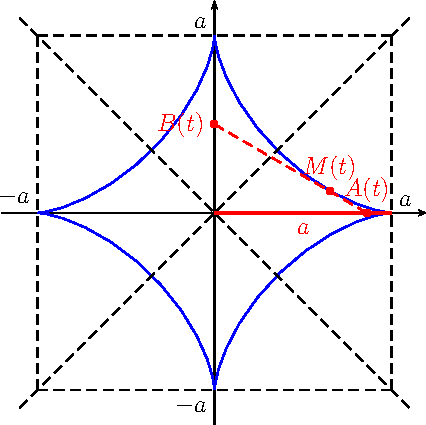
\includegraphics{../images/img005523-4}$$}
    \item \question{Pour $t\in]0,\frac{\pi}{2}[$, on note $A(t)$ et $B(t)$ les points d'intersection de la tangente au point
courant $M(t)$ avec respectivement $(Ox)$ et $(Oy)$. Calculer la longueur $A(t)B(t)$.}
\reponse{Soit $t\in\left]0,\frac{\pi}{2}\right[$. On a vu que la tangente $(T_t)$ en $M(t)$ est dirigée par le vecteur $(-\cos
t,\sin t)$. Une équation cartésienne de $T_t$ est donc : $-\sin t(x-a\cos^3t)-\cos t(y-a\sin^3t)=0$, ou encore

$$x\sin t+y\cos t=a\sin t\cos t\;(T_t).$$
On en déduit immédiatement que $A(t)$ a pour coordonnées $(a\cos t,0)$ et que $B(t)$ a pour coordonnées$(0,b\sin t)$
puis que

\begin{center}
\shadowbox{
$\forall t\in]0,\frac{\pi}{2}[,\;A(t)B(t)=a.$
}
\end{center}}
\end{enumerate}
}
